\chapter{Design and Implementation}
\section{Introduction}
Initially, when starting the development of this model, we looked at various tools and options to implement the model in code.  We settled on using Jupyter Notebooks along with a number of libraries to help make the development of this model easier and faster.  The useful thing about Jupyter Notebooks is that Jupyter Notebooks can be opened in a browser and all the code can be run from a single page.  We will detail the development of our proposed model both in this thesis and include notes in the notebook itself to explain my rationale behind implementing the model in a certain way.  During the initial phase of implementation, I used both the Keras documentation \cite{keras} and Tensorflow documentation \cite{tensorflow} as references to ensure that the model's development was following standard practices and to ensure that the model was optimized to allow training in a timely manner. 
\\
Due to the limited support for AMD graphics cards (currently the GPU in our system has a 6700XT which does not have RoCM support\cite{amdLimitations}) in a variety of popular AI frameworks/libraries at the time of writing this thesis, we decided it was best to use Google Colab Pro when training both the CNNs and the GANs this may offer some limitations in terms of memory and computational power.  Google Colab Pro, however, does offer a lot of advantages when it comes to quickly setting up an environment in which to train these models, it is for this reason that we have chosen to use it for training the models.
\\
For the purpose of reproducible results, we included the following lines of code \texttt{np.random.seed(9)} and set the random seed of Keras to 10 so that other researchers can reproduce similar results (achieving the same results depends on a number of factors) and build upon this study.  All the datasets are loaded and split using a seed of 1337 also so that the train/test split is the exact same every time.  Each model also uses a train / validation / test split of 70\% for train, 10\% for validation and 20\% for test(bar the chest X-ray COVID 19 dataset).  The rationale for having double the amount of data for the test set when compared with the validation set was made so that the test set could have more variety and therefore a higher degree of accuracy when comparing / contrasting the models.
\section{CNN Model Design and Comparison}
In this section we will compare and contrast each CNN's architecture and design when evaluating on both the original datasets and augmented datasets.  The goal of this section is to determine which architecture works best when creating the automated diagnostic system and whether or not the augmented dataset is increasing the model's generalization ability and the model's accuracy. Initially when training the models we thought about using early-stopping to improve the accuracy and reduce the loss of these models, we decided against this due to the harm it may cause the model's generalization ability.  All the models listed below use the entire data available when they are being trained.
\subsection{Baseline Models}
When starting the implementation phase, we decided to use the following resource to develop baseline CNN models \cite{imageClassificationKeras}.  We plan on modifying this resource to achieve a relatively high training/validation accuracy when training on the original dataset.  We plan on using these models to get a metric with which we can compare models generated on the original dataset to the models which are generated on the synthetic dataset.  It is in this way we can accurately compare the effects of the synthetic dataset on the accuracy of the implemented models.
\\
After this initial comparison is done with the models trained on the original dataset versus the models trained on the synthetic dataset.  We then plan on focusing on which architectures would work best when developing the CNN and how the models trained on the synthetic dataset can be improved.
\\
To start we decided to use the following settings when developing a CNN to be used when training on the x-ray COVID-19 dataset.  This dataset is made up of images that are labeled either 1 or 0 with 1 being COVID-positive and 0 being COVID-negative.  We have included the architecture of the layers of the model in the table below \ref{tab: X-ray COVID-19 dataset CNN baseline model architecture}
\begin{table}[H]
    \centering
    \resizebox{\textwidth}{!}{
    \begin{tabular}{|c|c|c|c|c|c|c|}
    \hline
        Layer Number 
        & Layer Type
        & Layer Size 
        & Kernel Size
        & Strides
        & Padding
        & Activation\\
        \hline
        1 & Conv2D Layer & 16 & (3,3) & 2 & Same & Swish\\
        2 & SeparableConv2D Layer & 32 & (3,3) & None & Same & Swish \\
        3  & SeparableConv2D Layer & 64 & (3,3) & None & Same & Swish \\
        4  & MaxPooling2D & 2 & 2 & None & Same & None \\
        5 & Residual & 64 & (3,3) & 2 & Same & Swish \\
        6 & SeparableConv2D & 128 & (3,3) & None & Same & Swish \\
        7 & GlobalAveragePooling2D & 1 & None & None & None & Sigmoid \\
        \hline
    \end{tabular}
        }
    \caption{ X-ray COVID-19 dataset CNN baseline model architecture}
    \label{tab: X-ray COVID-19 dataset CNN baseline model architecture}
\end{table}
For the padding the keyword ''same'' means that the input is padded with 0s evenly, both up and down and left and right of the image. The input was also scaled to normalize the data using the following line of code ''1.0 / 255)(inputs)''  After each layer batch normalization was performed excluding the residual, max pooling, and global average pooling 2D layers.  The use of the activation function ``swish`` was chosen due to studies showing it's performance matched or outperformed ReLU for certain tasks\cite{swishAndRelu}. Swish differs slightly in comparison to ReLU in that there isn't a sharp rise as the weight approaches 0. 
 \begin{figure}[H]
    \centering
    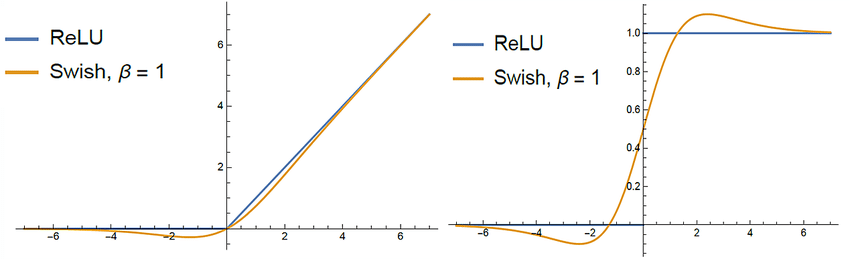
\includegraphics[width=1\textwidth,height=15cm,keepaspectratio]{Images/Swish ReLU activations.PNG}\\
    \caption{Figure of Swish and ReLU activation functions(Image courtesy of Madhura Ingalhalikar)\cite{swishReluDiagram}}
    \label{fig:Figure of Swish and ReLU activation functions}
\end{figure}
The model uses a dropout of 0, given the small size of the dataset we didn't want to drop neurons from the network. We also used the following settings when using model.compile() 
\begin{table}[H]
    \centering
    \resizebox{\textwidth}{!}{
    \begin{tabular}{|c|c|c|c|c|c|}
    \hline
         Optimizer
         & Loss Function 
         & Metric
         & Batch Size
         & Steps Per Epoch
         & Number of Epochs\\
         \hline
         Adam with a learning rate of $1\times10^{-3}$ & Binary CrossEntropy & Accuracy & 16 & 10 & 10\\
         \hline
    \end{tabular}
    }
    \caption{X-ray COVID-19 dataset CNN baseline model hyperparameters}
    \label{tab:X-ray COVID-19 dataset CNN baseline model hyperparameters}
\end{table}
The model was trained for a total of 37 epochs with 1 step per epoch (again due to the limitations in the size of the dataset) and achieved the following results.

\begin{table}[H]
    \centering
    \resizebox{\textwidth}{!}{
    \begin{tabular}{|c|c|c|c|c|c|}
    \hline
         Training Loss
         & Training Accuracy 
         & Validation Loss
         & Validation Accuracy
         & Test Set Loss
         & Test Set Accuracy\\
         \hline
         0.2651 & 0.9122 & 0.7918 & 0.5000 & 0.8173 & 0.4688\\
         \hline
    \end{tabular}
    }
    \caption{X-ray COVID-19 dataset CNN baseline model results}
    \label{tab:X-ray COVID-19 dataset CNN baseline model results}
\end{table}
 \begin{figure}[H]
    \centering
    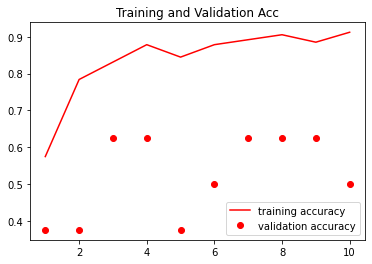
\includegraphics[width=1\textwidth,height=5cm,keepaspectratio]{Images/X-ray COVID-19 dataset CNN Train and Val Acc.png}\\
    \caption{Figure of Train and Validation Accuracy of X-ray COVID-19 dataset CNN Baseline Model  - The X-Axis shows the epoch number and the Y-axis shows the accuracy}
    \label{fig:X-ray COVID-19 dataset CNN Baseline Train and Validation Accuracy}
\end{figure}
 \begin{figure}[H]
    \centering
    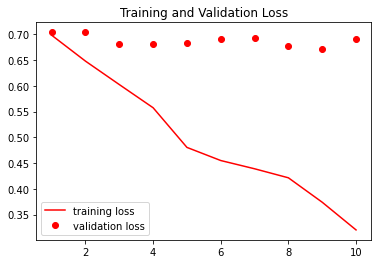
\includegraphics[width=1\textwidth,height=5cm,keepaspectratio]{Images/X-ray COVID-19 dataset CNN Train and Val Loss.png}\\
    \caption{Figure of Train and Validation Loss of X-ray COVID-19 dataset CNN Baseline Model  - The X-Axis shows the epoch number and the Y-axis shows the loss}
    \label{fig:X-ray COVID-19 dataset CNN Baseline Train and Validation Loss}
\end{figure}
As is shown from the results above \ref{tab:X-ray COVID-19 dataset CNN baseline model results} the model appears to be overfitting.  The model has a training accuracy which is 0.4122 higher than the validation accuracy.  The training loss is also much lower at 0.2651 when compared with the validation loss which is 0.7918.  The model overfitting the training set is expected given the small size of the dataset.  The model also performs very poorly on the test set and has a comparatively high loss and low accuracy when compared with the training set, which again is due to the limited data available.
\\
After finishing the CNN implementation for the X-ray COVID-19 dataset we then moved on to designing the model with the radiography dataset. This dataset is much larger than the original dataset, the radiography dataset contains a total of 30,306 image files broken into three classes.  In comparison, the X-ray COVID-19 dataset only contains 188 images belonging to two classes.  When designing this Convolutional network more thought had to be given to the split and which activation function to use for output, given that there are multiple classes.  When designing the CNN we decided to implement a much larger neural network given the amount of data available.  We tried using the initial network which was used for the X-ray COVID-19 dataset but the results were poor, increasing the size of the network led to better results.  Due to computational limitations we have decided to opt for ReLU instead of Swish as an activation function.
\begin{table}[H]
    \centering
    \resizebox{\textwidth}{!}{
    \begin{tabular}{|c|c|c|c|c|c|c|}
    \hline
        Layer Number 
        & Layer Type
        & Layer Size 
        & Kernel Size
        & Strides
        & Padding
        & Activation\\
        \hline
        1 & Conv2D Layer & 64 & (3,3) & 2 & Same & ReLU\\
        2 & SeparableConv2D Layer & 128 & (3,3) & 2 & Same & ReLU \\
        3  & SeparableConv2D Layer & 256 & (3,3) & 2 & Same & ReLU \\
        4 & SeparableConv2D Layer & 512 & (3,3) & 2 & Same & ReLU \\
        5  & MaxPooling2D & 3 & 2 & None & Same & None \\
        6 & Residual & 512 & (3,3) & 2 & Same & ReLU \\
        7 & SeparableConv2D & 1024 & (3,3) & None & Same & ReLU \\
        8 & GlobalAveragePooling2D & 3 & None & None & None & Softmax \\
        \hline
    \end{tabular}
    }
    \caption{Radiography CNN baseline model architecture}
    \label{tab:Radiography CNN baseline model architecture}
\end{table}


    \begin{table}[H]
    \centering
    \resizebox{\textwidth}{!}{
    \begin{tabular}{|c|c|c|c|c|c|}
    \hline
         Optimizer
         & Loss Function 
         & Metric
         & Batch Size
         & Steps Per Epoch
         & Number of Epochs\\
         \hline
         Adam with a learning rate of $1\times10^{-3}$ & sparse categorical crossentropy & Accuracy & 32 & 663 & 10\\
         \hline
    \end{tabular}
    }
    \caption{Radiography CNN baseline model hyperparameters}
    \label{tab:Radiography CNN baseline model hyperparameters}
\end{table}
In this model we achieved a higher accuracy when using ReLU as opposed to swift. The final results of the model are as follows:
\begin{table}[H]
    \centering
    \resizebox{\textwidth}{!}{
    \begin{tabular}{|c|c|c|c|c|c|}
    \hline
         Training Loss
         & Training Accuracy 
         & Validation Loss
         & Validation Accuracy
         & Test Set Loss
         & Test Set Accuracy\\
         \hline
         0.3446  & 0.8611 & 0.4120 & 0.8306 & 0.3800 & 0.8434\\
         \hline
    \end{tabular}
    }
    \caption{Radiography CNN baseline results}
    \label{tab:Radiography CNN baseline results}
\end{table}
 \begin{figure}[H]
    \centering
    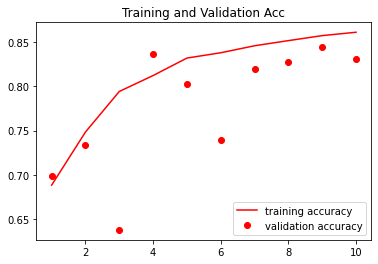
\includegraphics[width=1\textwidth,height=5cm,keepaspectratio]{Images/RadiographyCNNBaselineTrainAndValAcc.png}\\
    \caption{Train and Validation Accuracy of Radiography CNN Baseline Model - The X-Axis shows the epoch number and the Y-axis shows the accuracy}
    \label{fig:Radiography CNN Baseline Train and Validation Accuracy}
\end{figure}
 \begin{figure}[H]
    \centering
    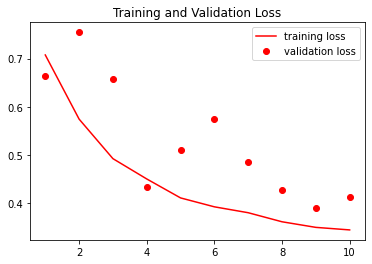
\includegraphics[width=1\textwidth,height=5cm,keepaspectratio]{Images/RadiographyCNNBaselineTrainAndValLoss.png}\\
    \caption{Figure of Train and Validation Loss of Radiography CNN Baseline Model - The X-Axis shows the epoch number and the Y-axis shows the loss}
    \label{fig:Second CNN Baseline Train and Validation Loss}
\end{figure}
As shown in the table \ref{tab:Radiography CNN baseline results} above we can see that the model has better results when compared with the first baseline model. One of the reasons for this is that we are dealing with a much larger dataset so the model has more images that it can learn features from, this yields a much higher accuracy when compared with the first baseline model which was trained on a much more limited dataset.
\\
The third baseline CNN model was trained using the COVID-19 chest X-ray dataset. This dataset didn't have a standardised resolution for images so the images had to be resized which could possibly lead to lack of data quality and consistency when resized.  For these models no test set was included as the some classes had very little data and it was impossible to include all classes when randomly sampling the data,  If data was manually included this would introduce bias so the test set was excluded from the model's evaluation.  When training the model there was a high degree of validation loss which is to be expected given the dataset size. The architecture of this model is as follows: 
\begin{table}[H]
    \centering
    \resizebox{\textwidth}{!}{
    \begin{tabular}{|c|c|c|c|c|c|c|}
    \hline
        Layer Number 
        & Layer Type
        & Layer Size 
        & Kernel Size
        & Strides
        & Padding
        & Activation\\
        \hline
        1 & Conv2D Layer & 32 & (3,3) & 2 & Same & Swish\\
        2 & SeparableConv2D Layer & 64 & (3,3) & 2 & Same & Swish \\
        3 & SeparableConv2D Layer & 128 & (3,3) & 2 & Same & Swish \\
        4 & SeparableConv2D Layer & 256 & (3,3) & 2 & Same & Swish \\
        5 & SeparableConv2D Layer & 512 & (3,3) & 2 & Same & Swish \\
        6  & MaxPooling2D & 3 & 2 & None & Same & None \\
        7 & Residual & 512 & (3,3) & 2 & Same & Swish \\
        8 & SeparableConv2D & 128 & (3,3) & None & Same & Swish \\
        9 & GlobalAveragePooling2D & 11 & None & None & None & Softmax \\
        \hline
    \end{tabular}
    }
    \caption{COVID-19 chest X-ray CNN baseline model architecture for COVID-19 Chest X-ray Dataset}
    \label{tab:COVID-19 chest X-ray CNN baseline model architecture}
\end{table}

    \begin{table}[H]
    \centering
    \resizebox{\textwidth}{!}{
    \begin{tabular}{|c|c|c|c|c|c|}
    \hline
         Optimizer
         & Loss Function 
         & Metric
         & Batch Size
         & Steps Per Epoch
         & Number of Epochs\\
         \hline
         Adam with a learning rate of $1\times10^{-3}$ & categorical crossentropy & Accuracy & 4 & 79 & 10\\
         \hline
    \end{tabular}
    }
    \caption{COVID-19 chest X-ray CNN baseline model hyperparameters for COVID-19 Chest X-ray Dataset}
    \label{tab:COVID-19 chest X-ray CNN baseline model hyperparameters}
\end{table}
Due to the small size of the dataset the batch size was set to a low number. The steps per epoch and number of epochs were also relatively low when compared with the other datasets due to the limited amount of data present.  The model's performance is shown in the table below:
\begin{table}[H]
    \centering
    \begin{tabular}{|c|c|c|c|}
    \hline
         Training Loss
         & Training Accuracy 
         & Validation Loss
         & Validation Accuracy\\
         \hline
         0.8372  & 0.7975 & 7.2848 & 0.6571\\
         \hline
    \end{tabular}
    \caption{COVID-19 chest X-ray CNN baseline model results for COVID-19 Chest X-ray Dataset}
    \label{tab:COVID-19 chest X-ray CNN baseline model results}
\end{table}
 \begin{figure}[H]
    \centering
    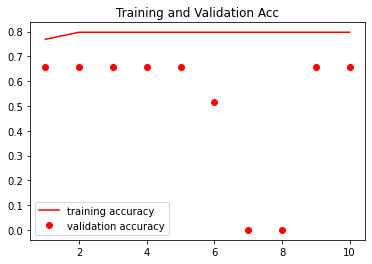
\includegraphics[width=1\textwidth,height=5cm,keepaspectratio]{Images/ChestXrayCNNBaselineTrainAndValAcc.png}\\
    \caption{Figure of Train and Validation Accuracy of COVID-19 chest X-ray CNN Baseline Model - The X-Axis shows the epoch number and the Y-axis shows the accuracy}
    \label{fig:COVID-19 chest X-ray CNN Baseline Train and Validation Accuracy}
\end{figure}
 \begin{figure}[H]
    \centering
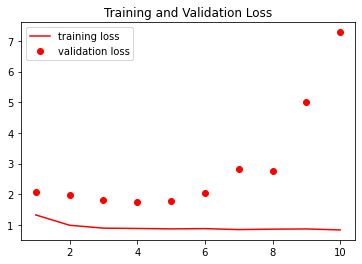
\includegraphics[width=1\textwidth,height=5cm,keepaspectratio]{Images/ChestXrayCNNBaselineTrainAndValLoss.png}\\
    \caption{Figure of Train and Validation Loss of COVID-19 chest X-ray CNN Baseline Model - The X-Axis shows the epoch number and the Y-axis shows the loss}
    \label{fig:COVID-19 chest X-ray CNN Baseline Train and Validation Loss}
\end{figure}
As shown in table \ref{tab:COVID-19 chest X-ray CNN baseline model results} the model has a high degree of loss and the accuracy isn't very good on either the training or the validation set.  This is to be expected as the dataset is quite small and contains a large number of classes.  The model suffers from insufficient data and has performed poorly due to data imbalance as well as lack of standardised image resolutions.
\\
The fourth and fifth baseline models were trained using the Extensive COVID Dataset.  This dataset is comprised of two different categories of images, one category of images being X-ray images and the other being CT scans.  Two different CNNs were trained, one was trained using the X-ray images and the other using the CT images.  The first baseline model for the Extensive COVID Dataset was trained on the CT images and the second baseline model was trained using the X-ray images.
\\
When creating the baseline model we trialled a number of different architectures the best performing of these architectures is shown in table \ref{tab:Extensive COVID-19 CT Dataset CNN Baseline Model Architecture}
\begin{table}[H]
    \centering
    \resizebox{\textwidth}{!}{
    \begin{tabular}{|c|c|c|c|c|c|c|}
    \hline
        Layer Number 
        & Layer Type
        & Layer Size 
        & Kernel Size
        & Strides
        & Padding
        & Activation\\
        \hline
        1 & Conv2D Layer & 32 & (3,3) & 2 & Same & ReLU\\
        2 & SeparableConv2D Layer & 64 & (3,3) & 2 & Same & ReLU \\
        3  & SeparableConv2D & 128 & None & None & Same & ReLU \\
        4 & SeparableConv2D & 256 & (3,3) & None & Same & ReLU \\
        5 & SeparableConv2D & 512 & (3,3) & None & Same & ReLU \\
        6 & residual & 512 & (3,3) & 2 & Same & ReLU \\
        7 & SeparableConv2D & 1024 & (3,3) & None & None & ReLU \\
        8 & activation layer & 1 & None & None & None & Sigmoid \\

        \hline
    \end{tabular}
    }
    \caption{Extensive COVID-19 CT Dataset CNN baseline model architecture}
    \label{tab:Extensive COVID-19 CT Dataset CNN Baseline Model Architecture}
\end{table}
\begin{table}[H]
    \centering
    \resizebox{\textwidth}{!}{
    \begin{tabular}{|c|c|c|c|c|c|}
    \hline
         Optimizer
         & Loss Function 
         & Metric
         & Batch Size
         & Steps Per Epoch
         & Number of Epochs\\
         \hline
         RMSprop with a learning rate of $1\times10^{-3}$ and a momentum of $1\times10^{-3}$ & binary crossentropy & Accuracy & 32 & 177 & 10\\
         \hline
    \end{tabular}
    }
    \caption{Extensive CT CNN baseline model hyperparameters}
    \label{tab:Extensive CT CNN baseline model hyperparameters}
\end{table}
\begin{table}[H]
    \centering
    \resizebox{\textwidth}{!}{
    \begin{tabular}{|c|c|c|c|c|c|}
    \hline
         Training Loss
         & Training Accuracy 
         & Validation Loss
         & Validation Accuracy
         & Test Set Loss
         & Test Set Accuracy\\
         \hline
         0.2286 & 0.9023 & 0.3837 & 0.8150 & 0.3574 & 0.8319\\
         \hline
    \end{tabular}
    }
    \caption{Extensive CT CNN baseline model results}
    \label{tab:Extensive CT CNN baseline model results}
\end{table}
The training / validation accuracy and loss for this model are visible in the images included below
 \begin{figure}[H]
    \centering
    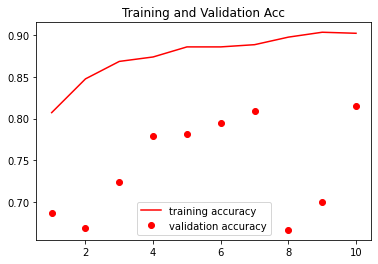
\includegraphics[width=1\textwidth,height=5cm,keepaspectratio]{Images/ExtensiveCNNBaselineModelExtensiveCovidAccCT.png}\\
    \caption{Figure of Train and Validation accuracy of Extensive COVID CNN Baseline Model CT  - The X-Axis shows the epoch number and the Y-axis shows the accuracy}
    \label{fig:Extensive COVID CT CNN Baseline Model CNN Baseline Train and Validation Accuracy}
\end{figure}
 \begin{figure}[H]
    \centering
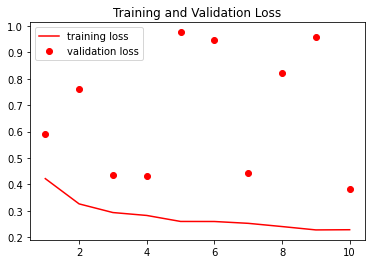
\includegraphics[width=1\textwidth,height=5cm,keepaspectratio]{Images/ExtensiveCNNBaselineModelExtensiveCovidLossCT.png}\\
    \caption{Figure of Train and Validation Loss of Extensive COVID CNN Baseline Model CT  - The X-Axis shows the epoch number and the Y-axis shows the loss}
    \label{fig:Extensive COVID CT CNN Baseline Model CNN Baseline Train and Validation Loss}
\end{figure}
When creating the baseline model we trialled a number of different architectures but found the following architecture detailed in table \ref{tab:Extensive COVID-19 X-Ray CNN Baseline Model Architecture}
\begin{table}[H]
    \centering
    \resizebox{\textwidth}{!}{
    \begin{tabular}{|c|c|c|c|c|c|c|}
    \hline
        Layer Number 
        & Layer Type
        & Layer Size 
        & Kernel Size
        & Strides
        & Padding
        & Activation\\
        \hline
        1 & Conv2D Layer & 32 & (3,3) & 2 & Same & ReLU\\
        2 & SeparableConv2D Layer & 64 & (3,3) & 2 & Same & ReLU \\
        3  & SeparableConv2D & 128 & None & None & Same & ReLU \\
        4 & SeparableConv2D & 256 & (3,3) & None & Same & ReLU \\
        5 & SeparableConv2D & 512 & (3,3) & None & Same & ReLU \\
        6 & residual & 512 & (3,3) & 2 & Same & ReLU \\
        7 & SeparableConv2D & 1024 & (3,3) & None & None & ReLU \\
        8 & activation layer & 1 & None & None & None & Sigmoid \\

        \hline
    \end{tabular}
    }
    \caption{Extensive COVID-19 X-Ray CNN Baseline Model Architecture}
    \label{tab:Extensive COVID-19 X-Ray CNN Baseline Model Architecture}
\end{table}
\begin{table}[H]
    \centering
    \resizebox{\textwidth}{!}{
    \begin{tabular}{|c|c|c|c|c|c|}
    \hline
         Optimizer
         & Loss Function 
         & Metric
         & Batch Size
         & Steps Per Epoch
         & Number of Epochs\\
         \hline
         RMSprop with a learning rate of $10^{-3}$ and a momentum of $10^{-3}$ & binary crossentropy & Accuracy & 32 & 209 & 10\\
         \hline
    \end{tabular}
    }
    \caption{Extensive COVID-19 X-Ray CNN baseline model hyperparameters}
    \label{tab:Extensive COVID-19 X-Ray CNN baseline model hyperparameters}
\end{table}
\begin{table}[H]
    \centering
    \resizebox{\textwidth}{!}{
    \begin{tabular}{|c|c|c|c|c|c|}
    \hline
         Training Loss
         & Training Accuracy 
         & Validation Loss
         & Validation Accuracy
         & Test Set Loss
         & Test Set Accuracy\\
         \hline
         0.1948 & 0.9278 & 0.3482 & 0.8587 & 0.3203 & 0.8698\\
         \hline
    \end{tabular}
    }
    \caption{Extensive COVID-19 X-Ray CNN baseline model results}
    \label{tab:Extensive COVID-19 X-Ray CNN baseline model results}
\end{table}
The training / validation accuracy and loss for this model are visible in the images included below
 \begin{figure}[H]
    \centering
    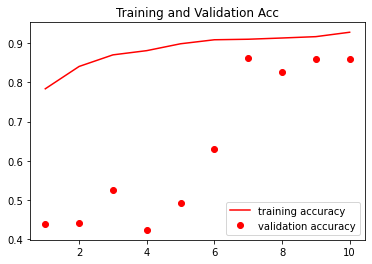
\includegraphics[width=1\textwidth,height=5cm,keepaspectratio]{Images/ExtensiveCOVID19XRayCNNBaselineModelAcc.png}\\
    \caption{Figure of Extensive COVID-19 X-ray CNN Baseline Model Train and Validation Accuracy - The X-Axis shows the epoch number and the Y-axis shows the accuracy}
    \label{fig:Extensive COVID-19 X-ray CNN Baseline ModelTrain and Validation Accuracy}
\end{figure}
 \begin{figure}[H]
    \centering
    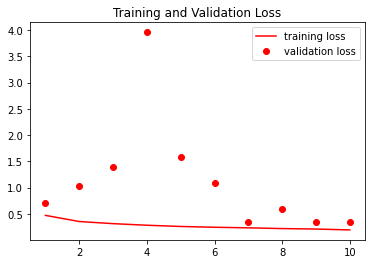
\includegraphics[width=1\textwidth,height=5cm,keepaspectratio]{Images/ExtensiveCOVID19XRayCNNBaselineModelLoss.png}\\
    \caption{Figure of Extensive COVID-19 X-ray CNN Baseline Model Train and Validation Loss  - The X-Axis shows the epoch number and the Y-axis shows the loss}
    \label{fig:Extensive COVID-19 X-ray CNN Baseline ModelTrain and Validation Loss}
\end{figure}
\section{Transfer Learning CNN Baseline Models}
Next we will compare the transfer learning baseline models. Keras offers a large number of pretrained models\cite{pretrainedModelsKeras}.  For the sake of time we have chosen the following three pretrained models to compare and contrast their effectiveness when automating COVID-19 diagnosis, Xception, ResNet50V2, and EfficientNetV2S were chosen as the architectures.  When choosing the pretrained models we had to carefully consider both their performance and size for use in this project.  Some models had parameters in excess of 100 million parameters which would not be usable in Colab Pro due to computational resource limitations.  Thus the models chosen had a reasonable number of parameters to avoid crashes when training the CNNs, the model with the highest number of parameters was ResNet50V2 which has 25.6M trainable parameters and the other two models have approximately 20 - 25 million parameters.  
\\
The weights used with all the transfer models come from models trained using the ImageNet dataset\cite{imageNet}.  The ImageNet dataset is comprised of 14,197,122 images and contains 1,000 classes.
\subsection{Radiography Dataset}
\subsubsection{Xception}
This model contains 21,386,795 parameters including a layer of 256 ReLU units and an additional layer of 3 softmax units which were appended to the model. The model ran for a total of 10 epochs with 663 steps per epoch.  The model also used sparse categorical cross entropy for the loss function and for the optimizer used Adam with a learning rate of $1\times10^{-3}$. The model achieved a final result of 0.9543 training accuracy with  0.1162  loss and had a validation accuracy of 0.8964 with a validation loss of 0.3867.  The model also has a test set accuracy of 0.9001 alongside a test set loss of 0.3833.  This is a relatively small but significant improvement in comparison to the original baseline models.  Figure \ref{fig:Transfer Learning Xception CNN Baseline Train and Validation Accuracy Radiography} shows the training and validation accuracy and figure \ref{fig:Transfer Learning Xception CNN Baseline Train and Validation Loss Radiography} shows the training and validation loss. 
 \begin{figure}[H]
    \centering
    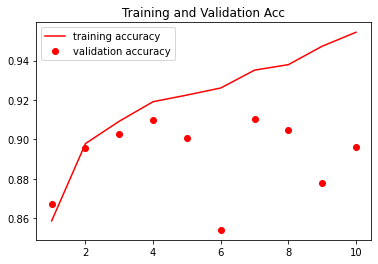
\includegraphics[width=1\textwidth,height=5cm,keepaspectratio]{Images/XceptionBaselineTrainingValidationAccRadiography.png}\\
    \caption{Transfer Learning Xception CNN Baseline Train and Validation Accuracy  - The X-Axis shows the epoch number and the Y-axis shows the accuracy}
    \label{fig:Transfer Learning Xception CNN Baseline Train and Validation Accuracy Radiography}
\end{figure}
 \begin{figure}[H]
    \centering    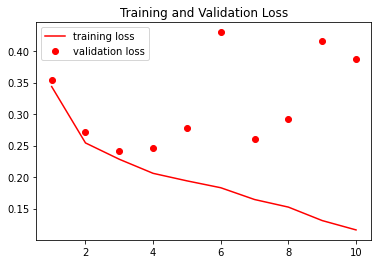
\includegraphics[width=1\textwidth,height=5cm,keepaspectratio]{Images/XceptionBaselineTrainingValidationLossRadiography.png}\\
    \caption{Transfer Learning Xception CNN Baseline Train and Validation Loss  - The X-Axis shows the epoch number and the Y-axis shows the loss}
    \label{fig:Transfer Learning Xception CNN Baseline Train and Validation Loss Radiography}
\end{figure}
\subsubsection{ResNet50V2}
This model had a total of 24,090,115 parameters including a layer of 256 ReLU units and an additional layer of 3 softmax units which were appended to the model.  This model had the same number of epochs and steps per epoch as exception(10 epochs with 663 steps) and also used the same optimizer with the same learning rate(Adam with $1\times10^{-3}$ as the learning rate).  The model performed slightly worse than Xception and finished with a training accuracy of 0.9172 and a training loss of 0.2024 and had a validation accuracy of 0.8695 with a validation loss of 0.3944.  The model also has a test set accuracy of 0.8809 and a test set loss of 0.3942.  Figure \ref{fig:Transfer Learning ResNet50V2 CNN Baseline Train and Validation Accuracy Radiography} shows the training and validation accuracy and figure \ref{fig:Transfer Learning ResNet50V2 CNN Baseline Train and Validation Loss Radiography} shows the training and validation loss. 
 \begin{figure}[H]
    \centering
    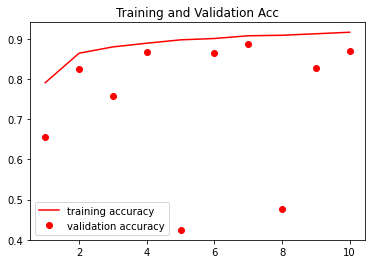
\includegraphics[width=1\textwidth,height=5cm,keepaspectratio]{Images/ResNet50V2BaselineTrainingValidationAccRadiography.png}\\
    \caption{Transfer Learning ResNet50V2 CNN Baseline Train and Validation Accuracy - The X-Axis shows the epoch number and the Y-axis shows the accuracy}
    \label{fig:Transfer Learning ResNet50V2 CNN Baseline Train and Validation Accuracy Radiography}
\end{figure}
 \begin{figure}[H]
    \centering
    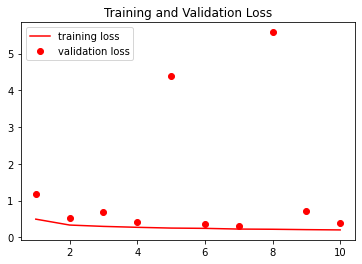
\includegraphics[width=1\textwidth,height=5cm,keepaspectratio]{Images/ResNet50V2BaselineTrainingValidationLossRadiography.png}\\
    \caption{Transfer Learning ResNet50V2 CNN Baseline Train and Validation Loss  - The X-Axis shows the epoch number and the Y-axis shows the loss}
    \label{fig:Transfer Learning ResNet50V2 CNN Baseline Train and Validation Loss Radiography}
\end{figure}
As shown in the figures above Xception outperforms this model when it comes to both the training accuracy and validation accuracy as well as the loss.
\subsubsection{EfficientNetV2S}
EfficientNetVS2 is a model with a total of 20,660,067 parameters including a layer of 256 ReLU units and an additional layer of 3 softmax units which were appended to the model.  Like the previous models this model was trained for a total of 10 epochs with 663 steps within each epoch.  It uses Adam as an optimizer with a learning rate of $1\times10^{-3}$.  The model performed worse than Xception but better than ResNet50V2 on the training,test, and validation sets. The model had a similar performance as Xception but managed to have a slightly lower train, test and validation accuracy and slightly lower losses for both the test and validation sets but a higher loss for the training set.  The model has a training accuracy of 0.9383 and a training loss of 0.1519 and a validation accuracy of 0.8844 and a validation loss of 0.3362.  The model also has a test loss of 0.3217 and a test accuracy of 0.8811. Figure \ref{fig:Transfer Learning EfficientNetV2S CNN Baseline Train and Validation Accuracy Radiography} shows the training and validation accuracy and figure \ref{fig:Transfer Learning EfficientNetV2S CNN Baseline Train and Validation Loss Radiography} shows the training and validation loss. 
 \begin{figure}[H]
    \centering
    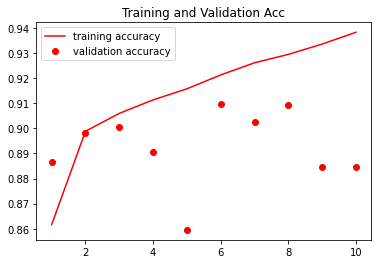
\includegraphics[width=1\textwidth,height=5cm,keepaspectratio]{Images/EfficientNetV2SBaselineTrainingValidationAccRadiography.png}\\
    \caption{Transfer Learning EfficientNetV2S CNN Baseline Train and Validation Accuracy  - The X-Axis shows the epoch number and the Y-axis shows the accuracy}
    \label{fig:Transfer Learning EfficientNetV2S CNN Baseline Train and Validation Accuracy Radiography}
\end{figure}
 \begin{figure}[H]
    \centering
    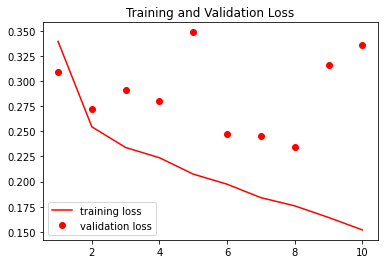
\includegraphics[width=1\textwidth,height=5cm,keepaspectratio]{Images/EfficientNetV2SBaselineTrainingValidationLossRadiography.png}\\
    \caption{Transfer Learning EfficientNetV2S CNN Baseline Train and Validation Loss  - The X-Axis shows the epoch number and the Y-axis shows the loss}
    \label{fig:Transfer Learning EfficientNetV2S CNN Baseline Train and Validation Loss Radiography}
\end{figure}
\subsection{X-Ray COVID-19 Dataset}
\subsubsection{Xception}
This model has a total of 22,960,681 parameters including a layer of 1024 ReLU units and a layer of 1 Sigmoid unit which were appended to the model. The model uses binary crossentropy as a loss function and uses Adam as an optimizer with a learning rate of $1\times10^{-3}$. 
The model ran for a total of 10 epochs with 10 steps per epoch.  The model achieved a training accuracy of 0.9662 with a training loss of 0.0951 and a validation accuracy of 0.5000 with a validation loss of 5.4697.  The model also had a test set loss of 7.5530 and a test set accuracy of 0.3750.  As with the baseline model this model is overfitting the training set which is to be expected given the small size of the dataset.  Figure \ref{fig:Xception CNN Baseline Train and Validation Accuracy X-Ray COVID19} shows the training and validation accuracy and figure \ref{fig:Xception CNN Baseline Train and Validation Loss X-Ray COVID19} shows the training and validation loss. 
 \begin{figure}[H]
    \centering
    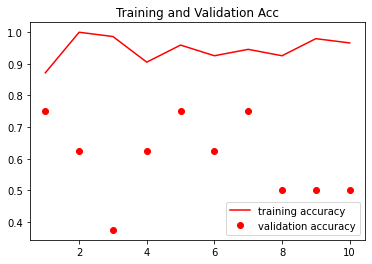
\includegraphics[width=1\textwidth,height=5cm,keepaspectratio]{Images/XceptionBaselineTrainingValidationAccuracyXRayCOVID19.png}\\
    \caption{Transfer Learning Xception CNN Baseline Train and Validation Accuracy X-Ray COVID19 - The X-Axis shows the epoch number and the Y-axis shows the accuracy}
    \label{fig:Xception CNN Baseline Train and Validation Accuracy X-Ray COVID19}
\end{figure}
 \begin{figure}[H]
    \centering
    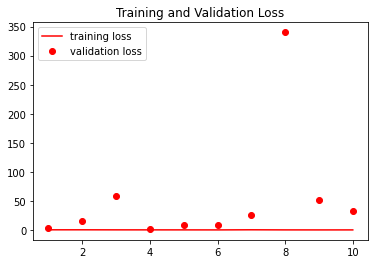
\includegraphics[width=1\textwidth,height=5cm,keepaspectratio]{Images/XceptionBaselineTrainingValidationLossXRayCOVID19.png}\\
    \caption{Transfer Learning Xception CNN Baseline Train and Validation Loss X-Ray COVID19 - The X-Axis shows the epoch number and the Y-axis shows the loss}
    \label{fig:Xception CNN Baseline Train and Validation Loss X-Ray COVID19}
\end{figure}
\subsubsection{ResNet50V2}
This model has a total of 25,664,001 parameters with an additional layer of 1024 ReLU units and another layer of 1 sigmoid unit which was appended to the model.  The model uses binary crossentropy as a loss function and Adam with a learning rate of $1\times10^{-3}$ as an optimizer.  The model ran for a total of 10 epochs with 10 steps per epoch and achieved a training accuracy of 0.9257 and a training loss of 0.2622 along with a validation accuracy of 0.3750 and a validation loss of 29.2193.  The model also has a high test loss of 23.9440 and an accuracy of 0.4688.  As with both the baseline and Xception models this model has overfit the training set. Figure \ref{fig:ResNet50V2 CNN Baseline Train and Validation Accuracy X-Ray COVID19} shows the training and validation accuracy and figure \ref{fig:ResNet50V2 CNN Baseline Train and Validation Loss X-Ray COVID19} shows the training and validation loss.
 \begin{figure}[H]
    \centering
    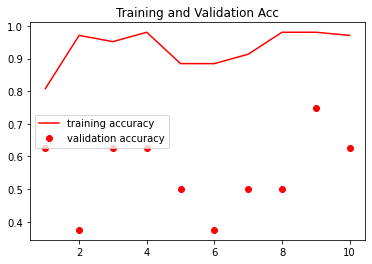
\includegraphics[width=1\textwidth,height=5cm,keepaspectratio]{Images/ResNet50V2BaselineTrainingValidationAccuracyXRayCOVID19.png}\\
    \caption{Transfer Learning ResNet50V2 CNN Baseline Train and Validation Accuracy X-Ray COVID19 - The X-Axis shows the epoch number and the Y-axis shows the accuracy}
    \label{fig:ResNet50V2 CNN Baseline Train and Validation Accuracy X-Ray COVID19}
\end{figure}
 \begin{figure}[H]
    \centering
    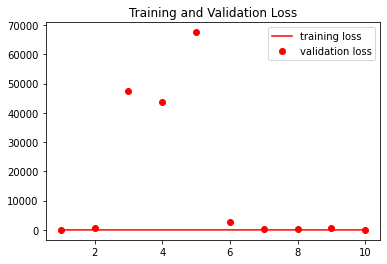
\includegraphics[width=1\textwidth,height=5cm,keepaspectratio]{Images/ResNet50V2BaselineTrainingValidationLossXRayCOVID19.png}\\
    \caption{Transfer Learning ResNet50V2 CNN Baseline Train and Validation Loss X-Ray COVID19 - The X-Axis shows the epoch number and the Y-axis shows the loss}
    \label{fig:ResNet50V2 CNN Baseline Train and Validation Loss X-Ray COVID19}
\end{figure}
\subsubsection{EfficientNetV2S}
This model has a total of 21,644,129 parameters with an additional layer of 1024 ReLU units and another layer of 1 sigmoid unit.  The model uses binary crossentropy as a loss funciton and Adam as an optimizer with a learning rate of $1\times10^{-3}$.  The model runs for a total of 10 epochs with 7 step per epoch. The model achieved a training accuracy of 1.000 with a training loss of 0.0063 and a validation accuracy of 1.0000 and a validation loss of 0.0011.  The model also achieved a test set loss of 0.2317 and a test set accuracy of 0.9375. Figure \ref{fig:EfficientNetV2S CNN Baseline Train and Validation Accuracy X-Ray COVID19} shows the training and validation accuracy and figure \ref{fig:EfficientNetV2S CNN Baseline Train and Validation Loss X-Ray COVID19} shows the training and validation loss. This model outperformed the baseline, Xception and ResNet50V2 models in terms of both loss and accuracy.
 \begin{figure}[H]
    \centering
    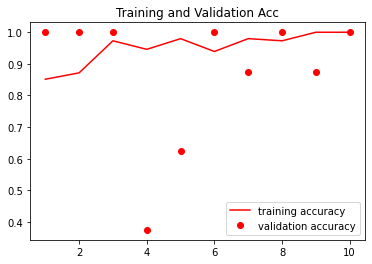
\includegraphics[width=1\textwidth,height=5cm,keepaspectratio]{Images/EfficientNetV2SBaselineTrainingValidationAccuracyXRayCOVID19.png}\\
    \caption{Transfer Learning EfficientNetV2S CNN Baseline Train and Validation Accuracy X-Ray COVID19 - The X-Axis shows the epoch number and the Y-axis shows the accuracy}
    \label{fig:EfficientNetV2S CNN Baseline Train and Validation Accuracy X-Ray COVID19}
\end{figure}
 \begin{figure}[H]
    \centering
    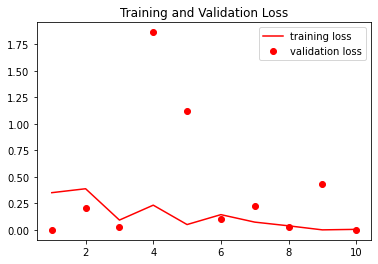
\includegraphics[width=1\textwidth,height=5cm,keepaspectratio]{Images/EfficientNetV2SBaselineTrainingValidationLossXRayCOVID19.png}\\
    \caption{Transfer Learning EfficientNetV2S CNN Baseline Train and Validation Loss X-Ray COVID19 - The X-Axis shows the epoch number and the Y-axis shows the loss}
    \label{fig:EfficientNetV2S CNN Baseline Train and Validation Loss X-Ray COVID19}
\end{figure}
\subsection{Evaluation of TL models for The x-ray covid 19 dataset}
The X-ray covid 19 dataset has a lack of data as it only comprises of 188 images.  It is not surprising to see that the models are greatly overfitting the training set.  Due to it's limited size this dataset may not be suitable for training GANs or the output of said GANs may lack diversity.
\subsection{COVID-19 Chest X-Ray Dataset}
\subsubsection{Xception}
This model has a total of 22,970,931 parameters including an additional layer of 1024 ReLU units and another layer of 11 softmax units which were appended to the model.  The model uses categorical crossentropy as a loss function along with Adam with a learning rate of $1 \times 10^{-3}$ as an optimizer.  The model runs for a total of 10 epochs with 79 step per epoch and achieved a training accuracy of 0.7975 and a training loss of 0.6109 along with a validation accuracy of 0.6571 and a validation loss of 1.6387. Figure \ref{fig:Xception CNN Baseline Train and Validation Accuracy Chest X-Ray} shows the training and validation accuracy and figure \ref{fig:Xception CNN Baseline Train and Validation Loss Chest X-Ray} shows the training and validation loss.
 \begin{figure}[H]
    \centering
    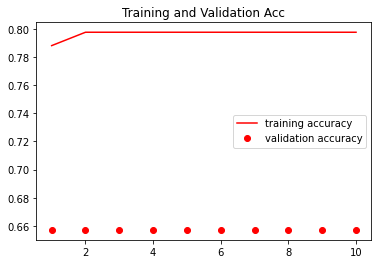
\includegraphics[width=1\textwidth,height=5cm,keepaspectratio]{Images/XceptionBaselineTrainingValidationAccuracyChestX-Ray.png}\\
    \caption{Transfer Learning Xception CNN Baseline Train and Validation Accuracy Chest X-Ray - The X-Axis shows the epoch number and the Y-axis shows the accuracy}
    \label{fig:Xception CNN Baseline Train and Validation Accuracy Chest X-Ray}
\end{figure}
 \begin{figure}[H]
    \centering
    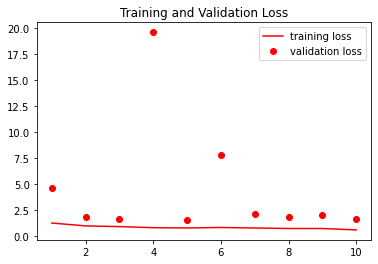
\includegraphics[width=1\textwidth,height=5cm,keepaspectratio]{Images/XceptionBaselineTrainingValidationLossChestX-Ray.png}\\
    \caption{Transfer Learning Xception CNN Baseline Train and Validation Loss X-Ray Chest X-Ray - The X-Axis shows the epoch number and the Y-axis shows the loss}
    \label{fig:Xception CNN Baseline Train and Validation Loss Chest X-Ray}
\end{figure}
\subsubsection{ResNet50V2}
This model has a total of 25,674,251 parameters including an additional layer of 1024 ReLU units and another layer of 11 softmax units which were appended to the model.  The model uses categorical crossentropy as a loss function along with Adam with a learning rate of $1 \times 10^{-3}$ as an optimizer.  The model runs for a total of 10 epochs with 79 step per epoch and achieved a training accuracy of 0.7975 and a training loss of 0.9676 along with a validation accuracy of 0.6571 and a validation loss of 1.5587. Figure \ref{fig:ResNet50V2 CNN Baseline Train and Validation Accuracy Chest X-Ray} shows the training and validation accuracy and figure \ref{fig:ResNet50V2 CNN Baseline Train and Validation Loss Chest X-Ray} shows the training and validation loss.
 \begin{figure}[H]
    \centering
    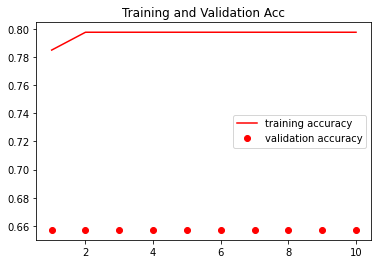
\includegraphics[width=1\textwidth,height=5cm,keepaspectratio]{Images/ResNet50V2BaselineTrainingValidationAccuracyChestX-Ray.png}\\
    \caption{Transfer Learning ResNet50V2 CNN Baseline Train and Validation Accuracy Chest X-Ray - The X-Axis shows the epoch number and the Y-axis shows the accuracy}
    \label{fig:ResNet50V2 CNN Baseline Train and Validation Accuracy Chest X-Ray}
\end{figure}
 \begin{figure}[H]
    \centering
    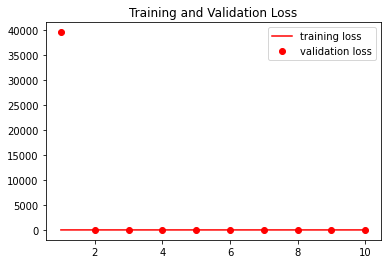
\includegraphics[width=1\textwidth,height=5cm,keepaspectratio]{Images/ResNet50V2BaselineTrainingValidationLossChestX-Ray.png}\\
    \caption{Transfer Learning ResNet50V2 CNN Baseline Train and Validation Loss X-Ray Chest X-Ray - The X-Axis shows the epoch number and the Y-axis shows the loss}
    \label{fig:ResNet50V2 CNN Baseline Train and Validation Loss Chest X-Ray}
\end{figure}
\subsubsection{EfficientNetV2S}
This model has a total of 21,654,379 parameters including an additional layer of 1024 ReLU units and another layer of 11 softmax units which were appended to the model.  The model uses categorical crossentropy as a loss function along with Adam with a learning rate of $1\times 10^{-2}$ as an optimizer.  The model runs for a total of 10 epochs with 79 step per epoch and achieved a training accuracy of 0.7975 and a training loss of 1.0280 along with a validation accuracy of 0.6571 and a validation loss of 1.7049. Figure \ref{fig:EfficientNetV2S CNN Baseline Train and Validation Accuracy Chest X-Ray} shows the training and validation accuracy and figure \ref{fig:EfficientNetV2S CNN Baseline Train and Validation Loss Chest X-Ray} shows the training and validation loss.
 \begin{figure}[H]
    \centering
    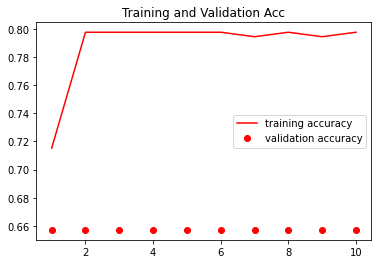
\includegraphics[width=1\textwidth,height=5cm,keepaspectratio]{Images/EfficientNetV2SBaselineTrainingValidationAccuracyChestX-Ray.png}\\
    \caption{Transfer Learning EfficientNetV2S CNN Baseline Train and Validation Accuracy Chest X-Ray - The X-Axis shows the epoch number and the Y-axis shows the accuracy}
    \label{fig:EfficientNetV2S CNN Baseline Train and Validation Accuracy Chest X-Ray}
\end{figure}
 \begin{figure}[H]
    \centering
    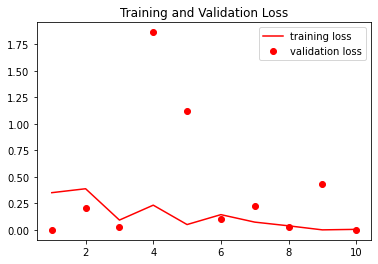
\includegraphics[width=1\textwidth,height=5cm,keepaspectratio]{Images/EfficientNetV2SBaselineTrainingValidationLossXRayCOVID19.png}\\
    \caption{Transfer Learning EfficientNetV2S CNN Baseline Train and Validation Loss Chest X-Ray - The X-Axis shows the epoch number and the Y-axis shows the loss}
    \label{fig:EfficientNetV2S CNN Baseline Train and Validation Loss Chest X-Ray}
\end{figure}
\subsection{Extensive COVID-19 Dataset CT}
\subsubsection{Xception}
This model is comprised of 21,386,281 parameters in total including an additional layer of 256 neurons using ReLU activation and an output layer of 1 neuron using a sigmoid activation function.  The model was trained for a total of 10 epochs with a total of 177 steps per epoch and uses RMSprop as an optimizer with a learning rate of $1\times10^{-3}$ and a momentum of $1\times10^{-3}$.  The model achieved a training accuracy of 0.9904 and a training loss of 0.0238 along with a validation accuracy of 0.9534 and a validation loss of 0.2250.  The model also had a test set loss of 0.1771 and a test accuracy of 0.9537. Figure \ref{fig:Xception CNN Baseline Train and Validation Accuracy Extensive COVID 19 Dataset CT} and figure \ref{fig:Xception CNN Baseline Train and Validation Loss Extensive COVID 19 Dataset CT} shows the training and validation loss.
 \begin{figure}[H]
    \centering
    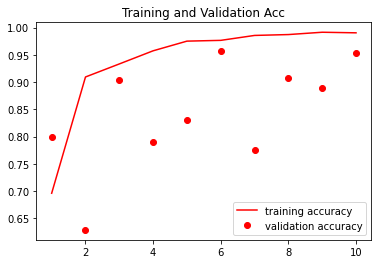
\includegraphics[width=1\textwidth,height=5cm,keepaspectratio]{Images/XceptionBaselineTrainingValidationAccuracyExtensiveCT.png}\\
    \caption{Transfer Learning Xception CNN Baseline Train and Validation Accuracy Extensive COVID 19 Dataset CT - The X-Axis shows the epoch number and the Y-axis shows the accuracy}
    \label{fig:Xception CNN Baseline Train and Validation Accuracy Extensive COVID 19 Dataset CT}
\end{figure}
 \begin{figure}[H]
    \centering
    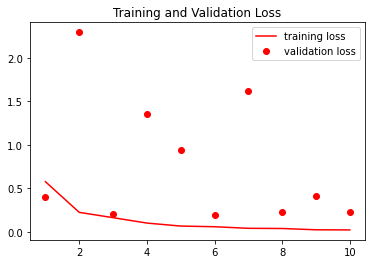
\includegraphics[width=1\textwidth,height=5cm,keepaspectratio]{Images/XceptionBaselineTrainingValidationLossExtensiveCT.png}\\
    \caption{Transfer Learning Xception CNN Baseline Train and Validation Loss Extensive COVID 19 Dataset CT - The X-Axis shows the epoch number and the Y-axis shows the loss}
    \label{fig:Xception CNN Baseline Train and Validation Loss Extensive COVID 19 Dataset CT}
\end{figure}
\subsubsection{ResNet50V2}
This model is comprised of 24,089,601 parameters in total including an additional layer of 256 neurons using ReLU activation and an output layer of 1 neuron using a sigmoid activation function.  The model was trained for a total of 10 epochs with 177 steps per epoch and uses RMSprop as an optimizer with a learning rate of $1\times10^{-3}$ and a momentum of $1\times10^{-3}$.  The model achieved a training accuracy of 0.9604 and a training loss of 0.1140 along with a validation accuracy of 0.9350 and a validation loss of 0.2078.  The model also has a test set accuracy of 0.9262 and a test set loss of 0.1993. Figure \ref{fig:ResNet50V2 CNN Baseline Train and Validation Accuracy Extensive COVID 19 Dataset CT} shows the training and validation accuracy and figure \ref{fig:ResNet50V2 CNN Baseline Train and Validation Accuracy Extensive COVID 19 Dataset CT} shows the training and validation loss.
 \begin{figure}[H]
    \centering
    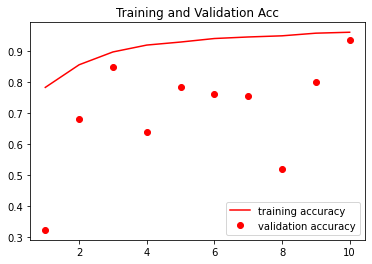
\includegraphics[width=1\textwidth,height=5cm,keepaspectratio]{Images/ResNet50V2BaselineTrainingValidationAccuracyExtensiveCT.png}\\
    \caption{Transfer Learning ResNet50V2 CNN Baseline Train and Validation Accuracy Extensive COVID 19 Dataset CT - The X-Axis shows the epoch number and the Y-axis shows the accuracy}
    \label{fig:ResNet50V2 CNN Baseline Train and Validation Accuracy Extensive COVID 19 Dataset CT}
\end{figure}
 \begin{figure}[H]
    \centering   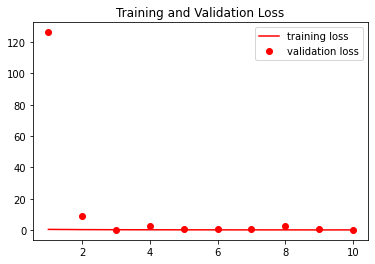
\includegraphics[width=1\textwidth,height=5cm,keepaspectratio]{Images/ResNet50V2BaselineTrainingValidationLossExtensiveCT.png}\\
    \caption{Transfer Learning ResNet50V2 CNN Baseline Train and Validation Loss Extensive COVID 19 Dataset CT - The X-Axis shows the epoch number and the Y-axis shows the loss}
    \label{fig:ResNet50V2 CNN Baseline Train and Validation Loss Extensive COVID 19 Dataset CT}
\end{figure}
\subsubsection{EfficientNetV2S}
This model is comprised of 20,659,553 parameters in total including an additional layer of 256 neurons using ReLU activation and an output layer of 1 neuron using a sigmoid activation function.  The model was trained for a total of 10 epochs with 177 steps per epoch and uses RMSprop as an optimizer with a learning rate of $1\times10^{-3}$ and a momentum of $1\times10^{-5}$.  The model achieved a training accuracy of 0.9901 and a training loss of 0.0291 along with a validation accuracy of 0.9375 and a validation loss of 0.2638.  The model also has a test set accuracy of 0.9438 and a test set loss of 0.2352. Figure \ref{fig:EfficientNetV2S CNN Baseline Train and Validation Accuracy Extensive COVID 19 Dataset CT} shows the training and validation accuracy and figure \ref{fig:EfficientNetV2S CNN Baseline Train and Validation Accuracy Extensive COVID 19 Dataset CT} shows the training and validation loss.
 \begin{figure}[H]
    \centering    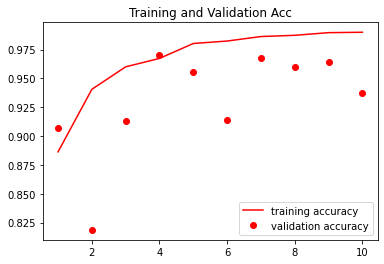
\includegraphics[width=1\textwidth,height=5cm,keepaspectratio]{Images/EfficientNetV2SBaselineTrainingValidationAccuracyExtensiveCT.png}\\
    \caption{Transfer Learning EfficientNetV2S CNN Baseline Train and Validation Accuracy Extensive COVID 19 Dataset CT - The X-Axis shows the epoch number and the Y-axis shows the accuracy}
    \label{fig:EfficientNetV2S CNN Baseline Train and Validation Accuracy Extensive COVID 19 Dataset CT}
\end{figure}
 \begin{figure}[H]
    \centering
    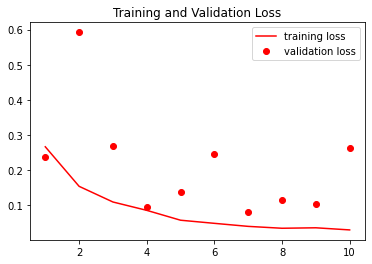
\includegraphics[width=1\textwidth,height=5cm,keepaspectratio]{Images/EfficientNetV2SBaselineTrainingValidationLossExtensiveCT.png}\\
    \caption{Transfer Learning EfficientNetV2S CNN Baseline Train and Validation Loss Extensive COVID 19 Dataset CT - The X-Axis shows the epoch number and the Y-axis shows the loss}
    \label{fig:EfficientNetV2S CNN Baseline Train and Validation Loss Extensive COVID 19 Dataset CT}
\end{figure}

\subsection{Extensive COVID-19 Dataset X-ray}
\subsubsection{Xception}
This model is comprised of 21,386,281 parameters in total including an additional layer of 256 neurons using ReLU activation and an output layer of 1 neuron using a sigmoid activation function.  The model was trained for a total of 10 epochs with a total of 177 steps per epoch and uses RMSprop as an optimizer with a learning rate of $1\times10^{-3}$ and a momentum of $1\times10^{-3}$.  The model achieved a training accuracy of 0.9876 and a training loss of 0.0277 along with a validation accuracy of 0.9416 and a validation loss of 0.2814.  The model also had a test set loss of 0.1947 and a test set accuracy of 0.9578. Figure \ref{fig:Xception CNN Baseline Train and Validation Accuracy Extensive COVID 19 Dataset X-ray} shows the training and validation accuracy and figure \ref{fig:Xception CNN Baseline Train and Validation Accuracy Extensive COVID 19 Dataset X-ray} shows the training and validation loss.
 \begin{figure}[H]
    \centering
    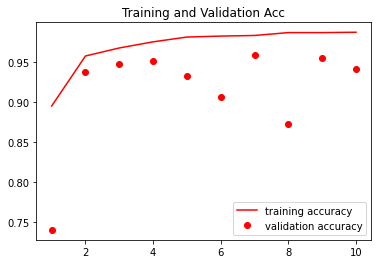
\includegraphics[width=1\textwidth,height=5cm,keepaspectratio]{Images/XceptionBaselineTrainingValidationAccuracyExtensiveXray.png}\\
    \caption{Transfer Learning Xception CNN Baseline Train and Validation Accuracy Extensive COVID 19 Dataset X-ray - The X-Axis shows the epoch number and the Y-axis shows the accuracy}
    \label{fig:Xception CNN Baseline Train and Validation Accuracy Extensive COVID 19 Dataset X-ray}
\end{figure}
 \begin{figure}[H]
    \centering
    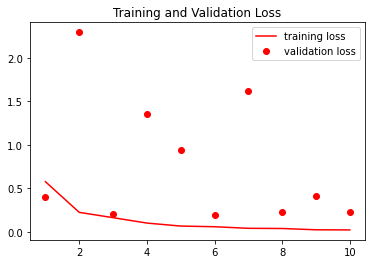
\includegraphics[width=1\textwidth,height=5cm,keepaspectratio]{Images/XceptionBaselineTrainingValidationLossExtensiveCT.png}\\
    \caption{Transfer Learning Xception CNN Baseline Train and Validation Loss Extensive COVID 19 Dataset X-ray - The X-Axis shows the epoch number and the Y-axis shows the loss}
    \label{fig:Xception CNN Baseline Train and Validation Loss Extensive COVID 19 Dataset X-ray}
\end{figure}
\subsubsection{ResNet50V2}
This model is comprised of 24,089,601 parameters in total including an additional layer of 256 neurons using ReLU activation and an output layer of 1 neuron using a sigmoid activation function.  The model was trained for a total of 10 epochs with 209 steps per epoch and uses RMSprop as an optimizer with a learning rate of $1\times10^{-3}$ and a momentum of $1\times10^{-3}$.  The model achieved a training accuracy of 0.9649 and a training loss of 0.0907 along with a validation accuracy of 0.9139 and a validation loss of 0.2842.  The model also has a test set accuracy of 0.9224 and a test set loss of 0.2379. Figure \ref{fig:ResNet50V2 CNN Baseline Train and Validation Accuracy Extensive COVID 19 Dataset X-ray} shows the training and validation accuracy and figure \ref{fig:ResNet50V2 CNN Baseline Train and Validation Loss Extensive COVID 19 Dataset X-ray} shows the training and validation loss.
 \begin{figure}[H]
    \centering
    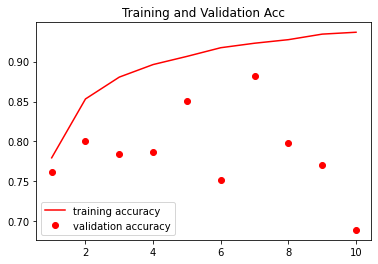
\includegraphics[width=1\textwidth,height=5cm,keepaspectratio]{Images/ResNet50V2BaselineTrainingValidationAccuracyExtensiveXray.png}\\
    \caption{Transfer Learning ResNet50V2 CNN Baseline Train and Validation Accuracy Extensive COVID 19 Dataset X-ray - The X-Axis shows the epoch number and the Y-axis shows the accuracy}
    \label{fig:ResNet50V2 CNN Baseline Train and Validation Accuracy Extensive COVID 19 Dataset X-ray}
\end{figure}
 \begin{figure}[H]
    \centering   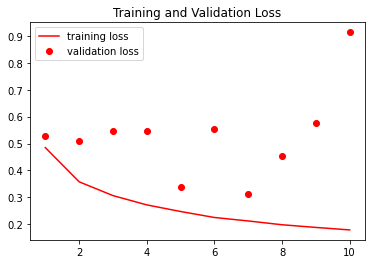
\includegraphics[width=1\textwidth,height=5cm,keepaspectratio]{Images/ResNet50V2BaselineTrainingValidationLossExtensiveXray.png}\\
    \caption{Transfer Learning ResNet50V2 CNN Baseline Train and Validation Loss Extensive COVID 19 Dataset X-ray - The X-Axis shows the epoch number and the Y-axis shows the loss}
    \label{fig:ResNet50V2 CNN Baseline Train and Validation Loss Extensive COVID 19 Dataset X-ray}
\end{figure}
\subsubsection{EfficientNetV2S}
This model is comprised of 20,659,553 parameters in total including an additional layer of 256 neurons using ReLU activation and an output layer of 1 neuron using a sigmoid activation function.  The model was trained for a total of 10 epochs with 209 steps per epoch and uses RMSprop as an optimizer with a learning rate of $1\times10^{-3}$ and a momentum of $1\times10^{-3}$.  The model achieved a training accuracy of 0.9840 and a training loss of 0.0396 along with a validation accuracy of 0.9702 and a validation loss of 0.2095.  The model also has a test set accuracy of 0.9766 and a test set loss of 0.1513.  Figure \ref{fig:EfficientNetV2S CNN Baseline Train and Validation Accuracy Extensive COVID 19 Dataset Xray} shows the training and validation accuracy and figure \ref{fig:EfficientNetV2S CNN Baseline Train and Validation Loss Extensive COVID 19 Dataset X-ray} shows the training and validation loss.
 \begin{figure}[H]
    \centering    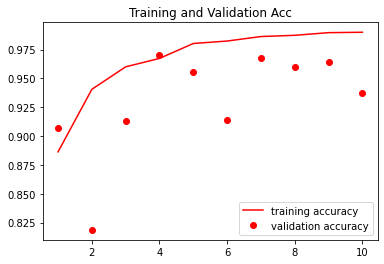
\includegraphics[width=1\textwidth,height=5cm,keepaspectratio]{Images/EfficientNetV2SBaselineTrainingValidationAccuracyExtensiveCT.png}\\
    \caption{Transfer Learning EfficientNetV2S CNN Baseline Train and Validation Accuracy Extensive COVID 19 Dataset X-ray - The X-Axis shows the epoch number and the Y-axis shows the accuracy}
    \label{fig:EfficientNetV2S CNN Baseline Train and Validation Accuracy Extensive COVID 19 Dataset Xray}
\end{figure}
 \begin{figure}[H]
    \centering
    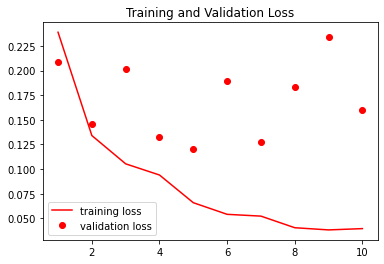
\includegraphics[width=1\textwidth,height=5cm,keepaspectratio]{Images/EfficientNetV2SBaselineTrainingValidationLossExtensiveXray.png}\\
    \caption{Transfer Learning EfficientNetV2S CNN Baseline Train and Validation Loss Extensive COVID 19 Dataset X-ray - The X-Axis shows the epoch number and the Y-axis shows the loss}
    \label{fig:EfficientNetV2S CNN Baseline Train and Validation Loss Extensive COVID 19 Dataset X-ray}
\end{figure}

\section{GAN Baseline Design and Comparison}
In this section we will detail the designs of the GANs and their architectures when augmenting classes in each database.  We will also compare the different results and effects each GAN architecture had when producing synthetic data.
\section{GANs for Radiography Dataset}
Due to a large imbalance between classes in the dataset we decided to explore the use of GANs to create synthetic data for both the COVID positive images which comprise 7,232 images in this dataset and the Pneumonia positive images which comprise 2,690 images.  The normal class (healthy patients) is very over-represented in the data as it is comprised of 20,384 images, due to this imbalance the CNNs trained from this dataset will be heavily biased towards identifying the normal patients.  For this reason we have chosen to use a number of Generative Adversarial Architectures to synthetically augment the classes lacking in data to balance the dataset and increase the generalization and robustness of the CNN models.
\subsection{VAE(Variational Auto Encoder)}
A few issues were encountered when running the variational auto encoder models for the radiography dataset.  When training on the masks we frequently ran into the issue of mode collapse, this is when the model only produces a single type of image.  Mode collapse occurred with both the COVID and Pneumonia datasets and can be seen below
 \begin{figure}[H]
    \centering
    
\includegraphics[width=1\textwidth,height=5cm,keepaspectratio]{Images/LatentSpace2VAECOVIDMask30Epochs.png}\\
    \caption{Example of Mode Collapse COVID Masks Radiography Dataset}
    \label{fig:Example of Mode Collapse COVID Masks Radiography Dataset}
\end{figure}
There were also issues faced when using a VAE on the X-ray data of both COVID and pneumonia images, the VAE tended to not produce any results when trained upon these X-rays and instead only showed a blank grid as output.  After a number of attempts to train both models it was found that the mask model suffered greatly from mode collapse and the X-ray model failed to produce any results for either class.
\subsection{DCGAN(Deep Convolutional GAN Network)}
\subsubsection{COVID-19 Mask Class Augmentation}
When designing the DCGAN we experimented with a number of architectures, some of these architectures led to the GAN only producing black squares which was a sign of mode collapse.  Mode collapse occurs when the discriminator gets stuck at a local minimum and the generator learns to only produce the same type of image over and over again to fool the discriminator. We found switching from an ADAM optimizer to RMSPROP and experimenting with the learning rate and momentum led to far better results.  The model produced some promising results, the following architecture was used to create the generator and discriminator:
\begin{minted}[linenos,tabsize=2,breaklines]{JavaScript}
# based off example: https://keras.io/examples/generative/dcgan_overriding_train_step/
discriminator = keras.Sequential(
    [
        keras.Input(shape=(128, 128, 3)),
        layers.Conv2D(64, kernel_size=4, strides=2, padding="same"),
        layers.LeakyReLU(alpha=0.5),
        layers.Conv2D(128, kernel_size=4, strides=2, padding="same"),
        layers.LeakyReLU(alpha=0.5),
        layers.Conv2D(128, kernel_size=4, strides=2, padding="same"),
        layers.LeakyReLU(alpha=0.5),
        layers.Flatten(),
        layers.Dropout(0.2),
        layers.Dense(1, activation="sigmoid"),
    ],
    name="discriminator",
)
discriminator.summary()

# Create the generator.
generator = keras.Sequential(
    [
        keras.Input(shape=(latent_dim,)),
        layers.Dense(8 * 8 * 128),
        layers.Reshape((8, 8, 128)),
        layers.Conv2DTranspose(256, kernel_size=4, strides=2, padding="same"),
        layers.LeakyReLU(alpha=0.2),
        layers.Conv2DTranspose(512, kernel_size=4, strides=2, padding="same"),
        layers.LeakyReLU(alpha=0.2),
        layers.Conv2DTranspose(1024, kernel_size=4, strides=2, padding="same"),
        layers.LeakyReLU(alpha=0.2),
        layers.Conv2DTranspose(64, kernel_size=4, strides=2, padding="same"),
        layers.LeakyReLU(alpha=0.2),
        layers.Conv2D(3, kernel_size=5, padding="same", activation="sigmoid"),
    ],
    name="generator",
)
generator.summary()
\end{minted}
The design of this GAN was based off of a Keras tutorial and the code was refactored for the purposes of this project\cite{DCGANKerasTutorial}.  The following hyper parameters were used when training the DCGAN model to generate synthetic COVID-19 mask images: 
\begin{table}[H]
    \centering
    \begin{tabular}{|c|c|}
    \hline
        Parameter
        & Value\\
         \hline
          Latent Dimension & 100\\
          Generator Optimizer & RMSProp \\
          Discriminator Optimizer & RMSProp\\
          Generator Learning Rate & $1\times10^{-5}$\\
          Discriminator Learning Rate & $1\times10^{-5}$\\
          Generator Momentum & 0\\
          Discriminator Momentum & 0\\
          Steps per Epoch & 452\\
          Batch Size & 8\\
          Number of Epochs & 100\\
         \hline
    \end{tabular}
    \caption{DCGAN for Producing Synthetic COVID-19 Mask Data From Radiography Dataset }
    \label{tab:DCGAN for Producing Synthetic COVID-19 Mask Data From Radiography Dataset}
\end{table}
With this model architecture we was able to achieve a final loss of 0.5476 for the discriminator and 1.0187 for the generator.
\subsubsection{COVID-19 X-Ray Class Augmentation}
Given the success achieved with the mask DCGAN we decided to reuse the architecture.  The results at first were blurry and had little resemblance to the actual data.  we decided to experiment with a number of different hyper parameters and found the parameters in the table below worked best:
\begin{table}[H]
    \centering
    \begin{tabular}{|c|c|}
    \hline
        Parameter
        & Value\\
         \hline
          Latent Dimension & 256\\
          Generator Optimizer & RMSProp \\
          Discriminator Optimizer & RMSProp\\
          Generator Learning Rate & $1\times10^{-5}$\\
          Discriminator Learning Rate & $1\times10^{-5}$\\
          Generator Momentum & 0\\
          Discriminator Momentum & 0\\
          Steps per Epoch & 452\\
          Batch Size & 8\\
          Number of Epochs & 100\\
         \hline
    \end{tabular}
    \caption{DCGAN for Producing Synthetic COVID-19 X-Ray Data From Radiography Dataset }
    \label{tab:DCGAN for Producing Synthetic COVID-19 X-Ray Data From Radiography Dataset}
\end{table}
With this model architecture we was able to achieve a final loss of 0.6859\% for the discriminator and 0.8015\% for the generator.
\subsubsection{Pneumonia Mask Class Augmentation}
The design of this DCGAN was based off the above COVID-19 DCGAN for generating masks and shares the same architecture the only difference being this model ran with 169 steps per epoch. The design yielded relatively similar results, although the losses for the pneumonia mask DCGAN was lower.  The model finished training with a loss of 0.9474 and a loss of 0.5936 for the discriminator.
\subsubsection{Pneumonia X-ray Class Augmentation}
The X-ray DCGAN for the pneumonia class is a copy of the above COVID-19 DCGAN the only difference being the Pneumonia X-Ray DCGAN uses a latent space of 256 and ran with 169 steps per epoch.  The model achieved a final loss of 0.6901 for the discriminator and a loss of 0.7534 for the generator.
\section{GANs for COVID 19 X-ray dataset}
\subsection{VAEs}
The decision was made not to train variational auto-encoders on this dataset given the poor performance of VAEs on the radiography dataset which is a lot larger than the X-ray COVID-19 dataset.  It appears that VAEs need much more data to train to recreate a similar image to the input data than the DCGAN models need.
\subsection{DCGANs}
There were some setbacks when training GANs on this dataset in particular due to the very limited amount of data it contained.  To remind the reader this dataset only contains 94 images of COVID-19 Positive X-Rays and 94 images of Pneumonia X-Rays.  When beginning the training of the GANs we merged both the train / test data for each class into two folders one marked Normal and the other marked Pneumonia each containing the 94 images of their respective class.  We merged both the test and the training data into the two files previously mentioned in order to utilize all the data available for augmenting the respective class. Most researchers suggest a minimum of 50k to 100k images to train a high quality GAN as mentioned on NVIDIAs website\cite{nvidiaResearch}. We attained some success with this DCGAN model surprisingly and augmented both the normal and pneumonia classes with 1,000 new images.
\\
The design of the DCGAN is as follows:
\begin{minted}[linenos,tabsize=2,breaklines]{JavaScript}
# based off example: https://keras.io/examples/generative/dcgan_overriding_train_step/
discriminator = keras.Sequential(
    [
        keras.Input(shape=(128, 128, 3)),
        layers.Conv2D(64, kernel_size=4, strides=2, padding="same"),
        layers.LeakyReLU(alpha=0.5),
        layers.Conv2D(128, kernel_size=4, strides=2, padding="same"),
        layers.LeakyReLU(alpha=0.5),
        layers.Conv2D(128, kernel_size=4, strides=2, padding="same"),
        layers.LeakyReLU(alpha=0.5),
        layers.Flatten(),
        layers.Dropout(0.4),
        layers.Dense(1, activation="sigmoid"),
    ],
    name="discriminator",
)
discriminator.summary()

# Create the generator.
generator = keras.Sequential(
    [
        keras.Input(shape=(latent_dim,)),
        layers.Dense(8 * 8 * 128),
        layers.Reshape((8, 8, 128)),
        layers.Conv2DTranspose(256, kernel_size=4, strides=2, padding="same"),
        layers.LeakyReLU(alpha=0.2),
        layers.Conv2DTranspose(512, kernel_size=4, strides=2, padding="same"),
        layers.LeakyReLU(alpha=0.2),
        layers.Conv2DTranspose(1024, kernel_size=4, strides=2, padding="same"),
        layers.LeakyReLU(alpha=0.2),
        layers.Conv2DTranspose(2048, kernel_size=4, strides=2, padding="same"),
        layers.LeakyReLU(alpha=0.2),
        layers.Conv2D(3, kernel_size=4, padding="same", activation="tanh"),
    ],
    name="generator",
)
generator.summary()

\end{minted}
The following hyper parameters were used to train the DCGAN to produce images from the normal class of the dataset
\begin{table}[H]
    \centering
    \begin{tabular}{|c|c|}
    \hline
        Parameter
        & Value\\
         \hline
          Latent Dimension & 256\\
          Generator Optimizer & RMSProp \\
          Discriminator Optimizer & RMSProp\\
          Generator Learning Rate & $1\times10^{-4}$\\
          Discriminator Learning Rate & $1\times10^{-4}$\\
          Generator Momentum & 0\\
          Discriminator Momentum & 0\\
          Steps per Epoch & 47\\
          Batch Size & 2\\
          Number of Epochs & 100\\
         \hline
    \end{tabular}
    \caption{DCGAN for Producing Synthetic Normal Class Data for X-ray COVID19 dataset}
    \label{tab:DCGAN for Producing Synthetic Normal Class Data for X-ray COVID19 dataset}
\end{table}
The final model achieved a loss of 0.6890 for the discriminator and a loss of 0.7623 for the generator.
\\
The augmentation of the pneumonia class had similar results as the normal class.  Given the success of the DCGAN architecture for the normal class it made sense to reuse this architecture when designing the DCGAN for the pneumonia class, the model also shares the same hyper-parameters.  The final model had a discriminator loss of 0.6895 and a generator loss of 0.7757 which is roughly around the same as the DCGAN for the normal class.
\section{GANs for Chest X-ray COVID-19}
Due to this model having 11 classes and limited data for each class a decision was made to exclude this dataset from the research.  This decision was made to conserve computational units and due to the limited data for each class.  There are also a number of classes in this dataset which contain very little data and are grossly underrepresented, the data for these classes is extremely limited and it would not be worthwhile training a GAN using this data.
\section{Extensive COVID-19 X-Ray / CT}
\subsection{VAEs}
The Extensive VAEs were trained on using both the X-ray COVID positive class and the Non-COVID CT class.  The output seemed to be fairly similar and it appears that the models suffered from mode collapse, but these images may have shown some benefit to the models.  The decision to conserve computational limits was made and the models were not augmented with data from the VAE models.  We have included images of the VAE models latent space below, as shown from the grids the resemblance between the images is striking although there may have been subtle differences non-descernible to the untrained eye.
 \begin{figure}[H]
    \centering
    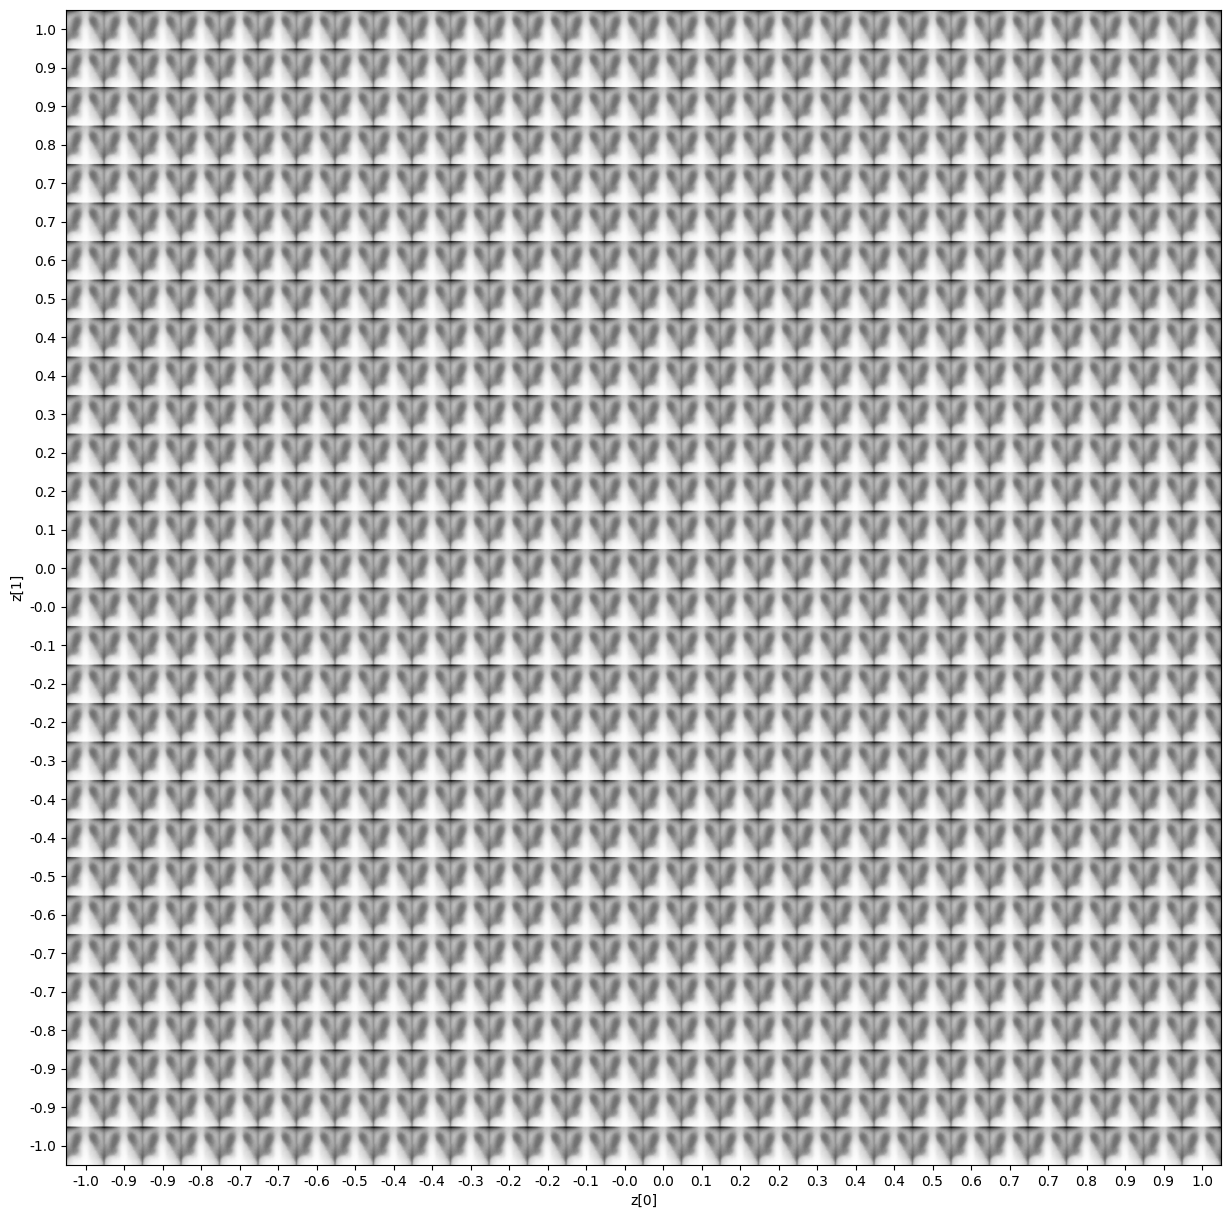
\includegraphics[width=1\textwidth,height=5cm,keepaspectratio]{Images/LatentSpaceExtensiveCOVIDXRay.png}\\
    \caption{Possible Mode Collapse COVID X-ray Extensive Dataset}
    \label{fig:Possible Mode Collapse COVID X-ray Extensive Dataset}
\end{figure}
 \begin{figure}[H]
    \centering
    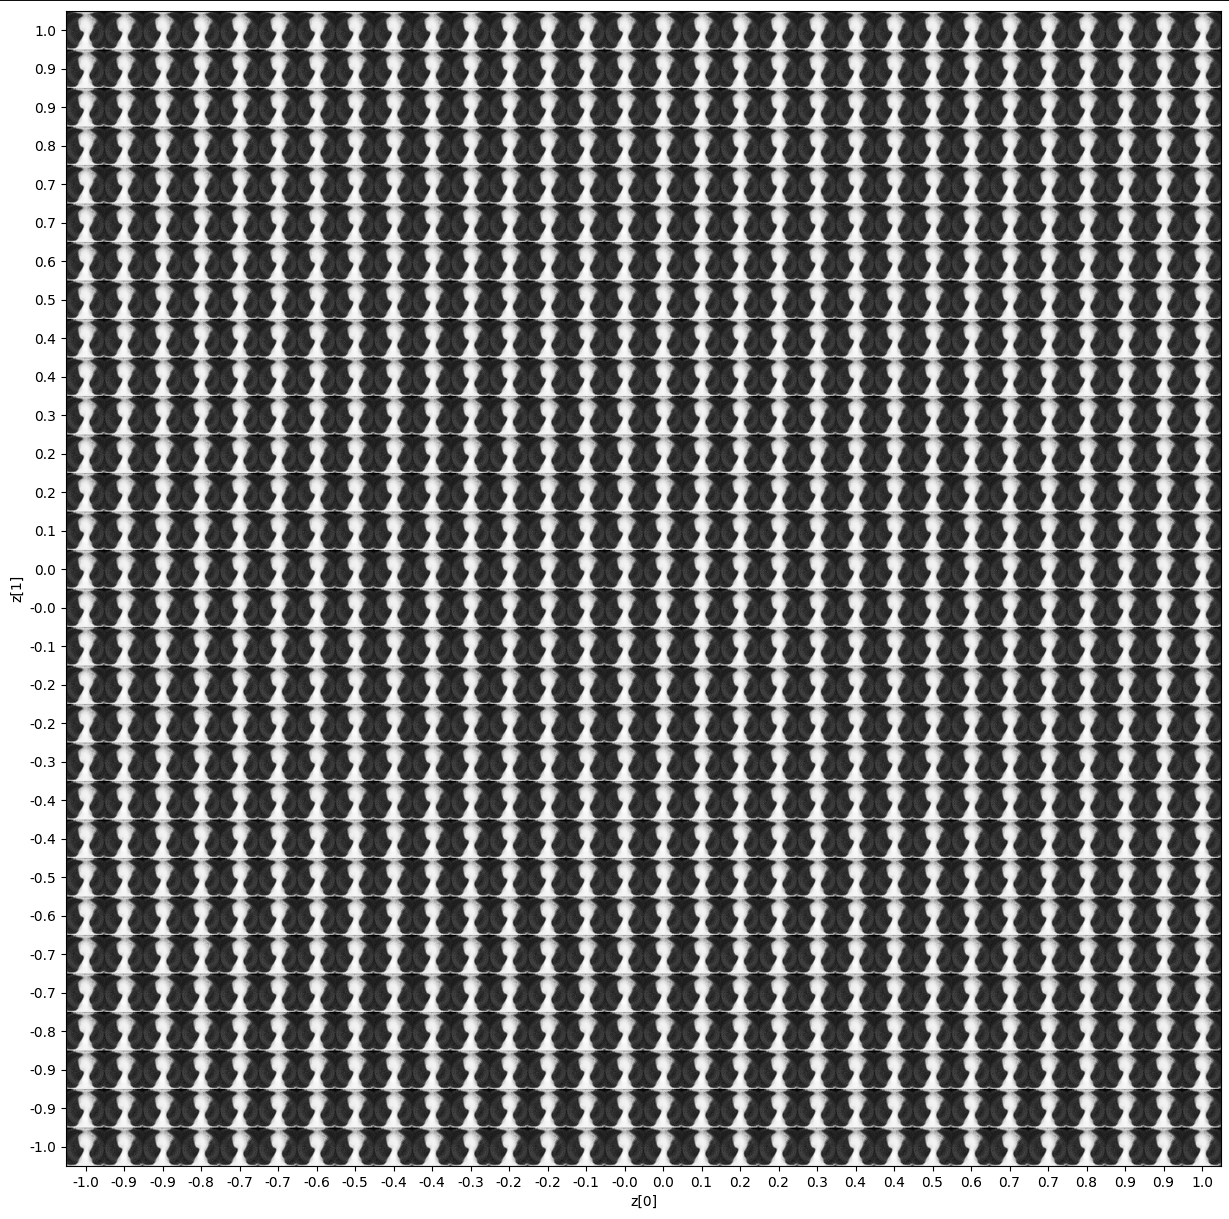
\includegraphics[width=1\textwidth,height=5cm,keepaspectratio]{Images/LatentSpaceExtensiveNonCovidCT.png}\\
    \caption{Possible Mode Collapse Non-Covid CT Extensive Dataset}
    \label{fig:Possible Mode Collapse Non-Covid CT Extensive Dataset}
\end{figure}
\subsection{DCGANs}
\subsubsection{X-ray DCGANs}
The extensive COVID-19 X-ray models were broken up into two classes COVID and Non-COVID.  The first model trained was trained to produce synthetic COVID images and ran for a total of 200 epochs and used the following architecture
\begin{minted}[linenos,tabsize=2,breaklines]{JavaScript}
# based off example: https://keras.io/examples/generative/dcgan_overriding_train_step/
discriminator = keras.Sequential(
    [
        keras.Input(shape=(128, 128, 3)),
        layers.Conv2D(64, kernel_size=4, strides=2, padding="same"),
        layers.LeakyReLU(alpha=0.5),
        layers.Conv2D(128, kernel_size=4, strides=2, padding="same"),
        layers.LeakyReLU(alpha=0.5),
        layers.Conv2D(128, kernel_size=4, strides=2, padding="same"),
        layers.LeakyReLU(alpha=0.5),
        layers.Flatten(),
        layers.Dropout(0.4),
        layers.Dense(1, activation="sigmoid"),
    ],
    name="discriminator",
)
discriminator.summary()

# Create the generator.
generator = keras.Sequential(A
    [
        keras.Input(shape=(latent_dim,)),
        layers.Dense(8 * 8 * 128),
        layers.Reshape((8, 8, 128)),
        layers.Conv2DTranspose(128, kernel_size=4, strides=2, padding="same"),
        layers.LeakyReLU(alpha=0.3),
        layers.Conv2DTranspose(256, kernel_size=4, strides=2, padding="same"),
        layers.LeakyReLU(alpha=0.3),
        layers.Conv2DTranspose(512, kernel_size=4, strides=2, padding="same"),
        layers.LeakyReLU(alpha=0.3),
        layers.Conv2DTranspose(1024, kernel_size=4, strides=2, padding="same"),
        layers.LeakyReLU(alpha=0.3),
        layers.Conv2D(3, kernel_size=4, padding="same", activation="tanh"),
    ],
    name="generator",
)
generator.summary()
\end{minted}
along with the following hyper parameters
\begin{table}[H]
    \centering
    \begin{tabular}{|c|c|}
    \hline
        Parameter
        & Value\\
         \hline
          Latent Dimension & 256\\
          Generator Optimizer & RMSProp \\
          Discriminator Optimizer & RMSProp\\
          Generator Learning Rate & $1\times10^{-4}$\\
          Discriminator Learning Rate & $1\times10^{-4}$\\
          Generator Momentum & 0\\
          Discriminator Momentum & 0\\
          Steps per Epoch & 253\\
          Batch Size &  16\\
          Number of Epochs & 200 \\
         \hline
    \end{tabular}
    \caption{DCGAN for Producing Synthetic X-ray COVID Class Data for Extensive COVID 19 Dataset}
    \label{tab:DCGAN for Producing Synthetic X-ray COVID Class Data for Extensive COVID 19 Dataset}
\end{table}
Once training finished the model attained a discriminator loss of 0.6901 and a generator loss of 0.7557.
\\ 
The next DCGAN architecture produced the Non-COVID class, this is the majority class but we wanted to compare and contrast the results from both DCGANs.  The model uses the following architecture 
\begin{minted}[linenos,tabsize=2,breaklines]{JavaScript}
# based off example: https://keras.io/examples/generative/dcgan_overriding_train_step/
discriminator = keras.Sequential(
    [
        keras.Input(shape=(128, 128, 3)),
        layers.Conv2D(64, kernel_size=4, strides=2, padding="same"),
        layers.LeakyReLU(alpha=0.5),
        layers.Conv2D(128, kernel_size=4, strides=2, padding="same"),
        layers.LeakyReLU(alpha=0.5),
        layers.Conv2D(128, kernel_size=4, strides=2, padding="same"),
        layers.LeakyReLU(alpha=0.5),
        layers.Flatten(),
        layers.Dropout(0.4),
        layers.Dense(1, activation="sigmoid"),
    ],
    name="discriminator",
)
# Create the generator.
generator = keras.Sequential(
    [
        keras.Input(shape=(latent_dim,)),
        layers.Dense(16 * 16 * 128),
        layers.Reshape((16, 16, 128)),
        layers.Conv2DTranspose(256, kernel_size=4, strides=2, padding="same"),
        layers.LeakyReLU(alpha=0.2),
        layers.Conv2DTranspose(512, kernel_size=4, strides=2, padding="same"),
        layers.LeakyReLU(alpha=0.2),
        layers.Conv2DTranspose(1024, kernel_size=4, strides=2, padding="same"),
        layers.LeakyReLU(alpha=0.2),
        layers.Conv2D(3, kernel_size=4, padding="same", activation="tanh"),
    ],
    name="generator",
)
\end{minted}
The model runs for 100 epochs and uses a learning rate of $10^{-5}$ for the generator and discriminator instead of $10^{-4}$.  The batch size was also increased to 64 to help the model train faster.  The model achieved a final loss of 0.6912 for the discriminator and 0.7575 for the generator.
\subsubsection{CT DCGANs}
For the DCGAN for CT Covid the batch size was chosen as 64 to increase the training speed.  The following architecture was used for this DCGAN
\begin{minted}[linenos,tabsize=2,breaklines]{JavaScript}
# based off example: https://keras.io/examples/generative/dcgan_overriding_train_step/
discriminator = keras.Sequential(
    [
        keras.Input(shape=(128, 128, 3)),
        layers.Conv2D(64, kernel_size=4, strides=2, padding="same"),
        layers.LeakyReLU(alpha=0.5),
        layers.Conv2D(128, kernel_size=4, strides=2, padding="same"),
        layers.LeakyReLU(alpha=0.5),
        layers.Conv2D(128, kernel_size=4, strides=2, padding="same"),
        layers.LeakyReLU(alpha=0.5),
        layers.Flatten(),
        layers.Dropout(0.4),
        layers.Dense(1, activation="sigmoid"),
    ],
    name="discriminator",
)
discriminator.summary()

# Create the generator.
generator = keras.Sequential(
    [
        keras.Input(shape=(latent_dim,)),
        layers.Dense(8 * 8 * 128),
        layers.Reshape((8, 8, 128)),
        layers.Conv2DTranspose(128, kernel_size=4, strides=2, padding="same"),
        layers.LeakyReLU(alpha=0.2),
        layers.Conv2DTranspose(256, kernel_size=4, strides=2, padding="same"),
        layers.LeakyReLU(alpha=0.2),
        layers.Conv2DTranspose(512, kernel_size=4, strides=2, padding="same"),
        layers.LeakyReLU(alpha=0.2),
        layers.Conv2DTranspose(1024, kernel_size=4, strides=2, padding="same"),
        layers.LeakyReLU(alpha=0.2),
        layers.Conv2D(3, kernel_size=4, padding="same", activation="tanh"),
    ],
    name="generator",
)
generator.summary()
\end{minted}
and used the following hyper parameters
\begin{table}[H]
    \centering
    \begin{tabular}{|c|c|}
    \hline
        Parameter
        & Value\\
         \hline
          Latent Dimension & 256\\
          Generator Optimizer & RMSProp \\
          Discriminator Optimizer & RMSProp\\
          Generator Learning Rate & $1\times10^{-4}$\\
          Discriminator Learning Rate & $1\times10^{-4}$\\
          Generator Momentum & 0\\
          Discriminator Momentum & 0\\
          Steps per Epoch & 85\\
          Batch Size &  64\\
          Number of Epochs & 100 \\
         \hline
    \end{tabular}
    \caption{DCGAN for Producing Synthetic CT COVID Class Data for Extensive COVID 19 Dataset}
    \label{tab:DCGAN for Producing Synthetic CT COVID Class Data for Extensive COVID 19 Dataset}
\end{table}
The model achieved a final loss score of 0.6443 for the discriminator and 0.9409 for the generator.
\\
The next model for the non-covid class uses the following architecture

\begin{minted}[linenos,tabsize=2,breaklines]{JavaScript}
# based off example: https://keras.io/examples/generative/dcgan_overriding_train_step/
discriminator = keras.Sequential(
    [
        keras.Input(shape=(128, 128, 3)),
        layers.Conv2D(64, kernel_size=4, strides=2, padding="same"),
        layers.LeakyReLU(alpha=0.5),
        layers.Conv2D(128, kernel_size=4, strides=2, padding="same"),
        layers.LeakyReLU(alpha=0.5),
        layers.Conv2D(128, kernel_size=4, strides=2, padding="same"),
        layers.LeakyReLU(alpha=0.5),
        layers.Flatten(),
        layers.Dropout(0.2),
        layers.Dense(1, activation="sigmoid"),
    ],
    name="discriminator",
)
discriminator.summary()

# Create the generator.
generator = keras.Sequential(
    [
        keras.Input(shape=(latent_dim,)),
        layers.Dense(4 * 4 * 128),
        layers.Reshape((4, 4, 128)),
        layers.Conv2DTranspose(64, kernel_size=4, strides=2, padding="same"),
        layers.LeakyReLU(alpha=0.2),
        layers.Conv2DTranspose(128, kernel_size=4, strides=2, padding="same"),
        layers.LeakyReLU(alpha=0.2),
        layers.Conv2DTranspose(256, kernel_size=4, strides=2, padding="same"),
        layers.LeakyReLU(alpha=0.2),
        layers.Conv2DTranspose(512, kernel_size=4, strides=2, padding="same"),
        layers.LeakyReLU(alpha=0.2),
        layers.Conv2DTranspose(1024, kernel_size=4, strides=2, padding="same"),
        layers.LeakyReLU(alpha=0.2),
        layers.Conv2D(3, kernel_size=4, padding="same", activation="tanh"),
    ],
    name="generator",
)
generator.summary()
\end{minted}
and the following hyper parameters 
\begin{table}[H]
    \centering
    \begin{tabular}{|c|c|}
    \hline
        Parameter
        & Value\\
         \hline
          Latent Dimension & 256\\
          Generator Optimizer & RMSProp \\
          Discriminator Optimizer & RMSProp\\
          Generator Learning Rate & $1\times10^{-4}$\\
          Discriminator Learning Rate & $1\times10^{-4}$\\
          Generator Momentum & 0\\
          Discriminator Momentum & 0\\
          Steps per Epoch & 42\\
          Batch Size &  64\\
          Number of Epochs & 100 \\
         \hline
    \end{tabular}
    \caption{DCGAN for Producing Synthetic CT Non COVID Class Data for Extensive COVID 19 Dataset}
    \label{tab:DCGAN for Producing Synthetic CT Non COVID Class Data for Extensive COVID 19 Dataset}
\end{table}
The model achieved a final loss score of 0.6522 for the discriminator and 1.0048 for the generator.
\section{Conclusion}
In conclusion most of the CNN models showed decent results when trained on the original datasets, although there are a few exceptions where the dataset used to train the models was small in size or imbalanced.  The GANs had achieved satisfactory results and produced images which were similar to those in the dataset which can be seen in the next chapter of this thesis.  Many of the models developed took a lot of tweaking, in order to get satisfactory results.  A lot of hyperparameter tuning was involved and the training was a time-consuming and laborious process as each model needed to be rerun when the hyperparameters were updated.
\\
With that said a number of models may benefit from more tweaking but for the purpose of this study the results achieved were satisfactory, given the purpose of this study is to gauge if synthetic data could improve an existing model's accuracy.  It is also worth remembering the models trained in this section are trained on limited data and/or imbalanced datasets which could skew the results. 

